% Preamble

\documentclass[a4paper]{article}


\usepackage[margin=1in]{geometry}

\usepackage{multicol}
\usepackage{lipsum}
\usepackage{hyperref}
\usepackage{natbib}
\usepackage{graphicx}
\usepackage{csquotes}





\begin{document}
    \author{Joschka Andersen}
    \date{\today{}}

    \title{Vorhersage der Busankunftszeiten der Flensburger Linienbusse}

    \maketitle


    \begin{abstract}
        Durch die öffentlich einsehbaren GPS-Daten der Flensburger Linienbusse, bereitgestellt unter
        https://www.busradar-flensburg.de/, bietet sich eine optimale Gelegenheit, diese Daten zu sammeln, um ein
        neuronales Netz zur Vorhersage der Ankunftszeiten zu trainieren.
        In dieser Arbeit geht es um das Sammeln dieser Daten, die Analyse und Vorverarbeitung sowie das Trainieren
        neuronaler Netze und die gewonnenen Erkenntnisse aus allen Stufen.
    \end{abstract}


    \section{Sammeln der Daten}
    \label{sec:sammeln-der-daten}

    \begin{figure}[h]
        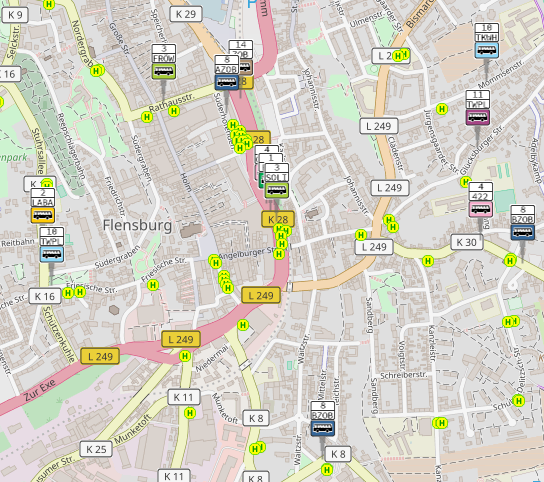
\includegraphics[scale=0.4]{figures/fig1_busradar}
        \centering
        \caption{Die Busradar-Webseite zeigt Live-Standortdaten der Linienbusse unter https://www.busradar-flensburg.de/}
        \label{fig:busradar}
    \end{figure}


    Die Busradar-Webseite\citep{busradarweb} bietet den Flensburgern einen Weg, live die Standorte aller Linienbusse
    nachzuverfolgen. Dabei greift die Webseite auf eine eigene API zu, bei der sie im 5-Sekunden-Takt neue Standortdaten
    anfragt. Die API stellt diese Daten im JSON-Format zur Verfügung. Sie beinhaltet für jedes Fahrzeug, welches Daten
    zur Verfügung stellt, Positionsdaten, Linien- und Zielinformationen, eine Fahrzeug-ID sowie einen Zeitstempel. Zudem
    werden auch alle Haltestellen mit Namen und Position in einer weiteren Anfrage zur Verfügung gestellt.

    Diese Daten sind der Kern dieser Arbeit und werden durch einen auf einem Server liegenden Crawler alle 3 Sekunden
    angefragt und in einer Datenbank gespeichert. Seit dem 23.11.2024 sammle ich so meine Daten und habe nun schon mehr
    als 2 GB an Rohdaten.


    \section{Analyse}
    \label{sec:analyse}


    Nach dem Sammeln der Daten habe ich angefangen mir der Daten bewusst zu werden und diese zuerst zu analysieren.
    Somit konnte ich Fehler im Datensatz ausfinding machen und auch überprüfen, ob meine Daten der wirklichkeit
    entsprechen. Mit der Datei analyse.ipynb ist die Analyse der Linie 14 enstanden.

    Die Analyse der Zielverteilung zeigte, dass, obwohl die Mehrheit der Daten korrekte Ziele und Linien aufweist,
    vereinzelt unsinnige Daten vorhanden sind. So gibt es beispielsweise in der Linie 14 auch Daten für die Linie 12,
    was bei mehreren Linien der Fall ist. Zudem wurden unsinnige Positionen mitten in Deutschland sowie fehlende oder
    negative Positionswerte festgestellt. Diese Erkenntnisse werden im Preprocessing verarbeitet, um Rauschen zu
    reduzieren. Darüber hinaus enthalten die Daten auch Leerfahrten und Schienenersatzverkehr, die in unserem
    Anwendungsfall wenig relevant sind. Da diese Daten nur selten vorkommen und keine nützlichen Informationen liefern,
    werden sie ebenfalls entfernt.


    \paragraph
    Durch eine visuelle Darstellung ist es mir gelungen, die Daten effektiv in Fahrten einzuteilen. Die Rohdaten gaben
    nur an, wann welcher Bus wo war, ohne eine Abgrenzung pro Fahrt. Eine Gruppierung in Fahrten ermöglicht mir jedoch
    eine bessere Vorverarbeitung, da ich nicht nur auf einzelne Punkte, sondern auf ganze Fahrten achten kann.

    Eine Darstellung\ref{fig:analyse} aller Einträge im Zeitverlauf eines Tages, gegenüber der Fahrzeug-ID sowie dem
    Ziel, zeigt, dass wir mit diesen drei Attributen die Daten erfolgreich in Fahrten aufteilen können.

    \begin{figure}[h]
        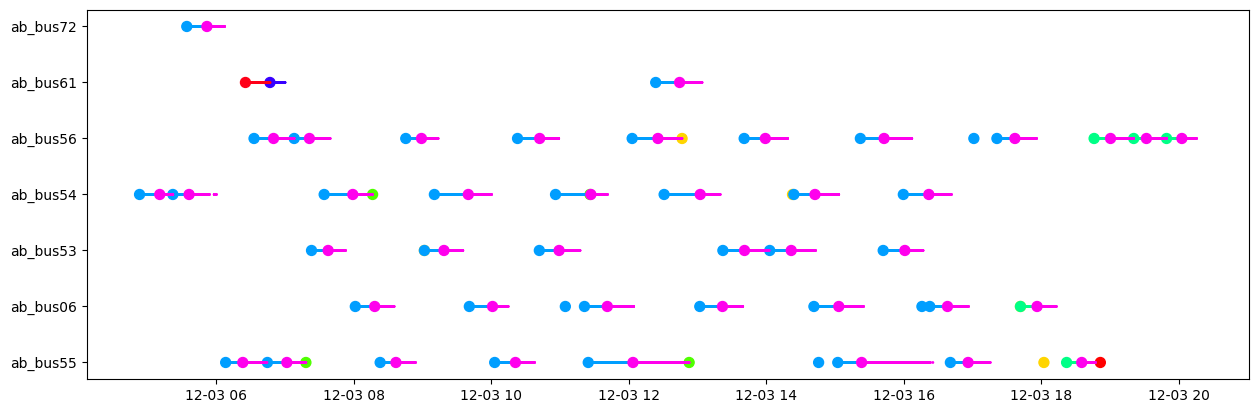
\includegraphics[scale=0.5]{figures/fig2_analyse}
        \centering
        \caption{Darstellung aller Einträge eines Tages von Linie 14 im Zeitverlauf, aufgeteilt in Fahrzeug-ID (x-Achse)
            sowie dem Ziel (Farbe). Die größeren Punkte entsprechen als Fahrtbeginn erkannte Trennpunkte.}
        \label{fig:analyse}
    \end{figure}


    Wenn wir nun nur alle Fahrtstartzeitpunkte dem Ziel gegenüberstellen, wie in Darstellung\ref{fig:analyse_intervall},
    können wir deutlich ein Intervall feststellen. Zudem ist farblich auch noch zu sehen, dass ab ca. kurz vor 18 Uhr
    die Fahrt nach FÖPA eine andere Strecke fährt. Berechnen wir den Durchschnittsabstand zwischen den Startpunkten,
    erhalten wir für die Richtung ZOB einen Wert von 21:13 Minuten und für Richtung FÖPA einen Wert von 19:54 Minuten.
    Vergleichen wir das mit dem Fahrplan, können wir verifizieren, dass unsere gesammelten Daten mit der Realität
    übereinstimmen.

    \begin{figure}[h]
        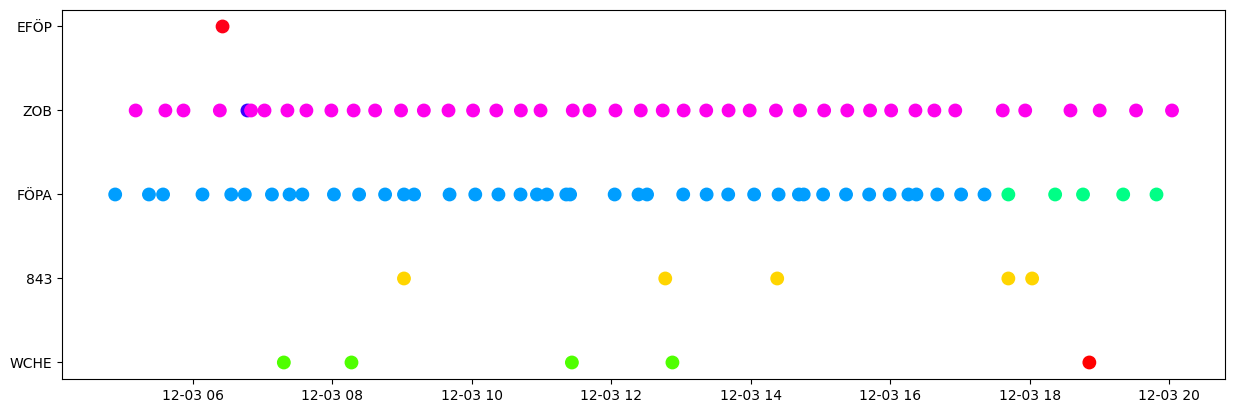
\includegraphics[scale=0.5]{figures/fig3_analyse_intervall}
        \centering
        \caption{Darstellung aller Startzeitpunkte eines Tages von Linie 14 gegenübergestellt dem generellen Ziel sowie
        der genauen Ziel-ID als Farbe.}
        \label{fig:analyse_intervall}
    \end{figure}


    Als weitere Analyse habe ich auch die Geschwindigkeit zwischen den einzelnen Punkten berechnet und alle Punkte
    markiert, an denen weniger als 5 km/h gefahren wird. Durch diese Analyse werden Kreuzungen und Haltestellen
    eindeutig erkennbar.


    \section{Vorverarbeitung}
    \label{sec:vorverarbeitung}

    Durch die Vorverarbeitung bringe ich meine selbst gesammelten Rohdaten in ein Format, mit dem ich die Netze
    trainieren möchte. Dabei liegt der Fokus auf dem Filtern von Rauschen sowie dem Gruppieren von Fahrten zu Strecken,
    um irrelevante Daten aus dem Training auszuschließen. Zudem entsprechen die in den Rohdaten vorhandenen Labels wie
    Ziel und Linie nicht unbedingt der Realität. Durch die Vorverarbeitung generiere ich mir diese Labels mittels
    verschiedener Clustering methoden. Die Vorverarbeitung erfolgt in mehreren Schritten und ist im
    preprocessing-Ordner zu finden. Um das Preprocessing selbst auszuführen, folge der README-Datei im
    genannten Ordner.

    Zunächst werden die Rohdaten gefiltert, sodass nur valide Daten innerhalb Flensburgs erhalten bleiben. Diese werden
    mit eindeutigen Fahrt-IDs versehen.

    Zusätzlich wird eine Datei erzeugt, die jede Fahrt mit Start- und Endpunkt definiert, um die Fahrten anschließend
    mithilfe von Clustering-Algorithmen zu gruppieren.

    \subsection{Basisstrecken}
    \label{subsec:basisstrecken}

    Jetzt geht es darum, aus dem Datensatz Basisstrecken zu identifizieren. Diese repräsentieren eine Strecke und sollen
    genutzt werden, um alle Fahrten einer Strecke zuzuordnen.

    Um eindeutige Strecken zu ermitteln, werden die Start- und Endpositionen mittels DBSCAN\cite{ester1996dbscan}
    gruppiert. DBSCAN\cite{ester1996dbscan} ist ein density-based Clustering-Verfahren, das die Start- und Endpositionen
    anhand ihrer Dichte zueinander gruppiert.

    \begin{figure}[h]
        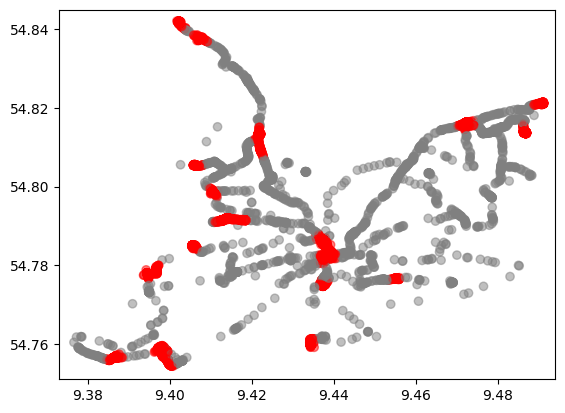
\includegraphics[scale=0.5]{figures/fig4_vorverarbeitung_start_cluster}
        \centering
        \caption{Gruppierte Startpositionen. In Rot alle unterschiedlichen Gruppen und in Grau alle nicht zugehörigen
        Punkte.}
        \label{fig:start_cluster}
    \end{figure}

    Wie in Darstellung\ref{fig:start_cluster} veranschaulicht, werden Strecken mit häufig genutzten Start- und
    Endpositionen beibehalten. Fahrten, die außerhalb oder mitten auf der Strecke starten, werden herausgefiltert. Alle
    Fahrten sind nun nach der Kombination aus Start- und Endposition gruppiert.

    Um die Strecken besser zu validieren und zu benennen, nutze ich meine Haltestellendatei in Kombination mit einem
    KD-Tree-Algorithmus\cite{kdtree} für eine schnelle nearest-neighbor-Suche.

    Anschließend filtere ich alle Gruppen mit mehr als 100 Fahrten. Ich überprüfe die erkannten Strecken anhand der im
    Datensatz vorhandenen Linien. Während die meisten Strecken nur ein oder zwei Linienwerte aufweisen, gibt es bei
    einigen mehrere, was vor allem als Rauschen in den Daten erkennbar ist. Auffällig ist, dass viele verschiedene
    Fahrten zur oder von der Haltestelle \textit{Balastbrücke} führen.

    Für jede Gruppe erstelle ich eine Distanzmatrix, in der jede Fahrt innerhalb der Gruppe mit jeder anderen verglichen
    wird. Um die Distanz zwischen zwei Fahrten zu bestimmen, werden diese zunächst mithilfe des
    Douglas-Peucker-Algorithmus\cite{douglaspeucker} mit einem Epsilon-Wert von 0.001 vereinfacht. Anschließend berechne
    ich die Distanzen der vereinfachten Versionen mittels Dynamic Time Warping\cite{dtw} und speichere sie als Matrix.

    Im nächsten Schritt verwende ich ein flaches Clustering\cite{modernhierachical}, um mithilfe der Distanzmatrizen
    Gruppen anhand ähnlicher Fahrten zu erstellen. Aus der größten Gruppe wird anschließend eine zufällig ausgewählte
    Fahrt als Basis-Referenzfahrt bestimmt. Diese definiert die Strecke.

    Durch die verschiedenen Verarbeitungsschritte wird sichergestellt, dass als Referenzstrecke nur Fahrten gewählt
    werden, die am häufigsten vorkommen. Dadurch haben Baustellen, Straßensperrungen und temporäre Verkehrsänderungen
    keinen Einfluss auf die Auswahl der Referenzstrecke.

    \subsection{Gruppierung und Trainingsdaten}
    \label{subsec:gruppierung}

    Anhand der Referenzstrecken wird mithilfe des Douglas-Peucker-Algorithmus\cite{douglaspeucker} zur Vereinfachung
    und Dynamic Time Warping\cite{dtw} zum Vergleich eine kleine Distanzmatrix erstellt. In dieser werden alle im
    Datensatz enthaltenen Fahrten anhand eines Schwellenwerts einer Gruppe zugeordnet.

    Im letzten Schritt vor dem Trainieren werden aus den gesäuberten und gruppierten Daten Datensätze erstellt, die ich
    relativ einfach in meinen neuronalen Netzen verwenden kann. In meinen ersten Versuchen habe ich die Haltestellen
    genutzt, um für eine Linie durch die Positionsdaten die Ankunft an allen Haltestellen vorherzusagen. Diese Variante
    hat jedoch ziemlich schlecht performt, mit einem MSE-Loss von ca. 20, und ist sehr starr auf eine Linie angewiesen.

    Meine aktuelle Herangehensweise versucht, das Netz mit zwei Positionen zu fragen: \enquote{Wann wirst du an Position
    zwei ankommen, wenn du jetzt bei Position eins bist?}. Dazu erstelle ich zu jeder Fahrt 200 Paare mit beiden
    Positionen sowie den zugehörigen Zeitpunkten. Zusätzlich gebe ich die bisherige Durchschnittsgeschwindigkeit, die
    bisher gefahrene Zeit und die bisher gefahrene Strecke als zusätzliche Informationen zur ersten Position. Ich
    benutze ein Limit von 200 Paaren pro Fahrt, um meinen Datensatz nicht explodieren zu lassen, da ich pro Fahrt
    $n^2$ viele Paare bilden könnte. Mit 200 Paaren erstelle ich nur einen Datensatz mit $4,5$ Millionen Einträgen.

    
    Zudem erstelle ich einen Train/Validation-Split, der anhand von Fahrten aufgeteilt wird. Dadurch werden keine 
    Teilstücke aus einer Fahrt in beiden Trainings- und Validierungsdaten enthalten sein. Ich nutze einen Split von 
    70/30. Da die Anzahl der Fahrten pro Gruppe in meinem Datensatz nicht ausgewogen ist, splitte ich meinen Datensatz 
    für jede Gruppe separat mit einem 70/30-Verhältnis. Leider ist mir erst sehr spät aufgefallen, dass die Inbalance 
    einen negativen Effekt auf mein Training haben könnte. Alle trainierten Netze wurden mit diesem Datensatz trainiert. 
    Im Folgenden\ref{fig:gruppen_verteilung} ist die normalisierte Verteilung der Gruppen im Trainings- und
    Validierungssplit zu sehen.
    
    \begin{figure}[h]
        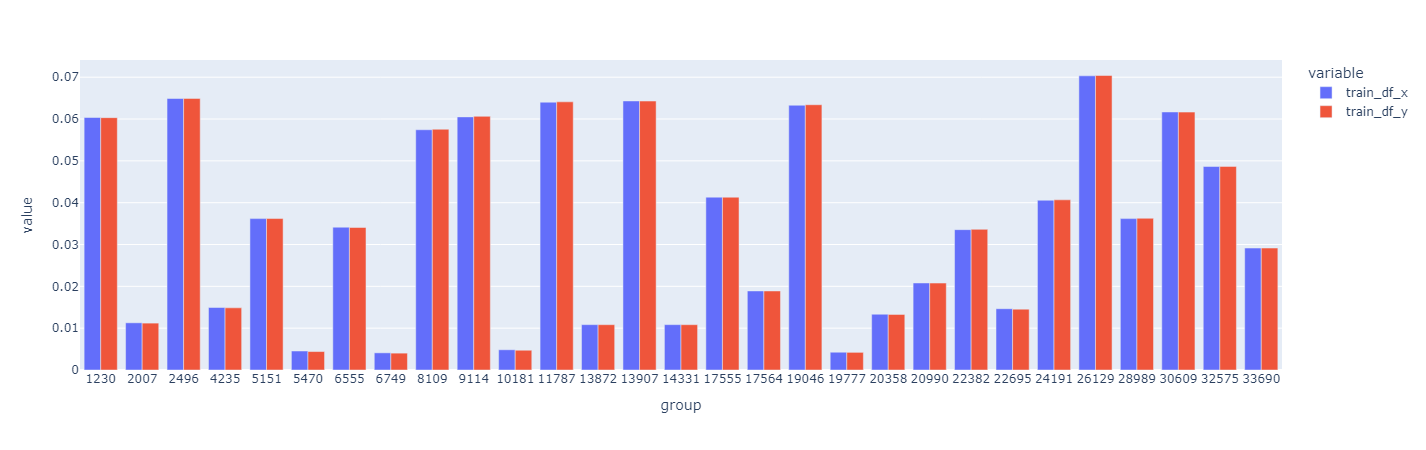
\includegraphics[scale=0.35]{figures/fig5_gruppen_verteilung}
        \centering
        \caption{Gruppenverteilung im Validierungs und Trainingsdatensplit}
        \label{fig:gruppen_verteilung}
    \end{figure}


    \section{Training}
    \label{sec:training}

    Im Training habe ich zwei verschiedene MLP und verschiedenen Inputsdaten Trainiert und mit einander verglichen.

    \begin{figure}[h]
        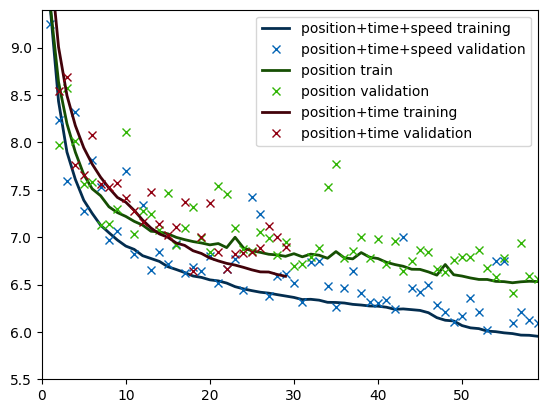
\includegraphics[scale=0.6]{figures/fig6_training_different_input_data}
        \centering
        \caption{Trainieren mit gleichem complexem MLP jedoch mit Zeit und Durchschnittsgeschwindigkeit}
        \label{fig:training_different_input}
    \end{figure}

    \begin{figure}[h]
        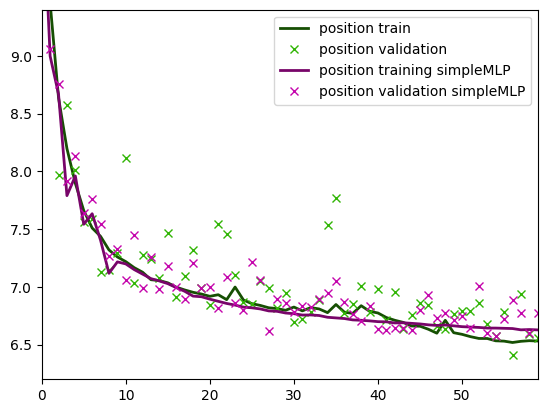
\includegraphics[scale=0.6]{figures/fig7_training_different_mlp_complexity}
        \centering
        \caption{Trainieren mit nur der Position jedoch unterschiedlicher MLP complexity}
        \label{fig:training_different_complexity}
    \end{figure}

    \begin{figure}[h]
        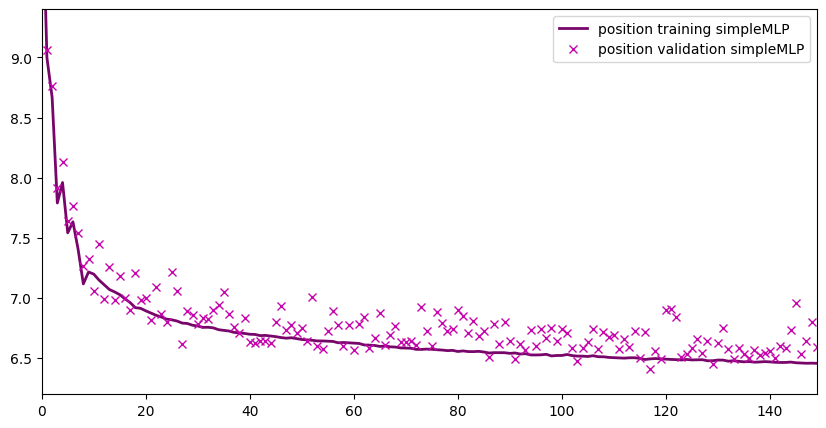
\includegraphics[scale=0.6]{figures/fig8_training_simpler_mlp}
        \centering
        \caption{Ganzes Training des einfachen MLPs}
        \label{fig:training_simpler_mlp}
    \end{figure}





    \bibliographystyle{plain}
    \begin{thebibliography}{10}

        \bibitem{busradarweb}
        https://www.busradar-flensburg.de/

        \bibitem{ester1996dbscan}
        Martin Ester, Hans-Peter Kriegel, Jörg Sander, Xiaowei Xu
        \newblock A Density-Based Algorithm for Discovering Clusters in Large Spatial Databases with Noise
        \newblock In *Proceedings of the Second International Conference on Knowledge Discovery and Data Mining (KDD-96)*, pages 226–231, 1996.

        \bibitem{kdtree}
        Songrit Maneewongvatana, David M. Mount
        \newblock Analysis of approximate nearest neighbor searching with clustered point sets
        \newblock {\em arXiv arXiv:cs/9901013}, 1999.

        \bibitem{douglaspeucker}
        David Douglas, Thomas Peucker
        \newblock Algorithms for the reduction of the number of points required to represent a digitized line or its caricature.
        \newblock In *The Canadian Cartographer*. Band 10, Nr. 2, 1973.

        \bibitem{dtw}
        Donald J. Berndt, James Clifford
        \newblock Using dynamic time warping to find patterns in time series.
        \newblock In *AAAIWS'94: Proceedings of the 3rd International Conference on Knowledge Discovery and Data Mining*, pages 359-370, 1994.

        \bibitem{modernhierachical}
        Daniel Müller
        \newblock Modern hierarchical, agglomerative clustering algorithms
        \newblock {\em arXiv arXiv:1109.2378}, 2011.

    \end{thebibliography}


\end{document}